\documentclass[]{article}
\usepackage{graphicx}
\usepackage{hyperref}

%opening
\title{Introduction to Machine Learning Final Project}
\author{Paula Campaña Donoso $-$ 730723162 \\ Brad Weyand $-$ 730318989 \\ Siwei Han $-$ 730723179 \\ Thomas Kung $-$ 730620459}

\begin{document}

\maketitle

\begin{abstract}
For this project, the idea is to guess between poisonous and non-poisonous mushrooms using binary classification as well as random forests. The dataset that was chosen provides numerous categories for the different aspects of each type of mushroom. There is around 23 species of mushrooms inside this data set, and 23 categories in which this mushorooms are being classified. The first 22 categories help distinguish the characteristics of each of the mushrooms, while the last category determines whether or not the mushroom can be considered poisonous or not. There is a prepocessing section to change the data from strings to integers, then a visualization of the data. After that, the model is being trained and finally the accuracy of the model is being tested in order to see the results from this analysis.
\end{abstract}

\section{Pre-Processing Data}

\textbf{How was it done?}
\medskip

In order to use the data set for the analysis to guess whether or not the mushrooms are poisounous, the data set needed to be pre-processed to change all the categorical classifications that were registered as strings, into integers. For that reason we started by investigating which could be the best approach to transform the information in order to have a better result for the random forest model. After some research, it was determined that we would have to change the values using One-Hot encoding process. This process would allow us ot have all the classifications in binary outputs $(0,1)$. With this new classification form, we can be able to interpret the data better as there would not be factors such as ranking that interfere in our guessing of the poisonous level of each of the mushrooms, and also it is a form of data interpretation that allows the random forests analyze the data easily and better.

\section{Visualization}
The following image contains different set of graphs that show each category.

\begin{figure}[!htb]
	\centering
	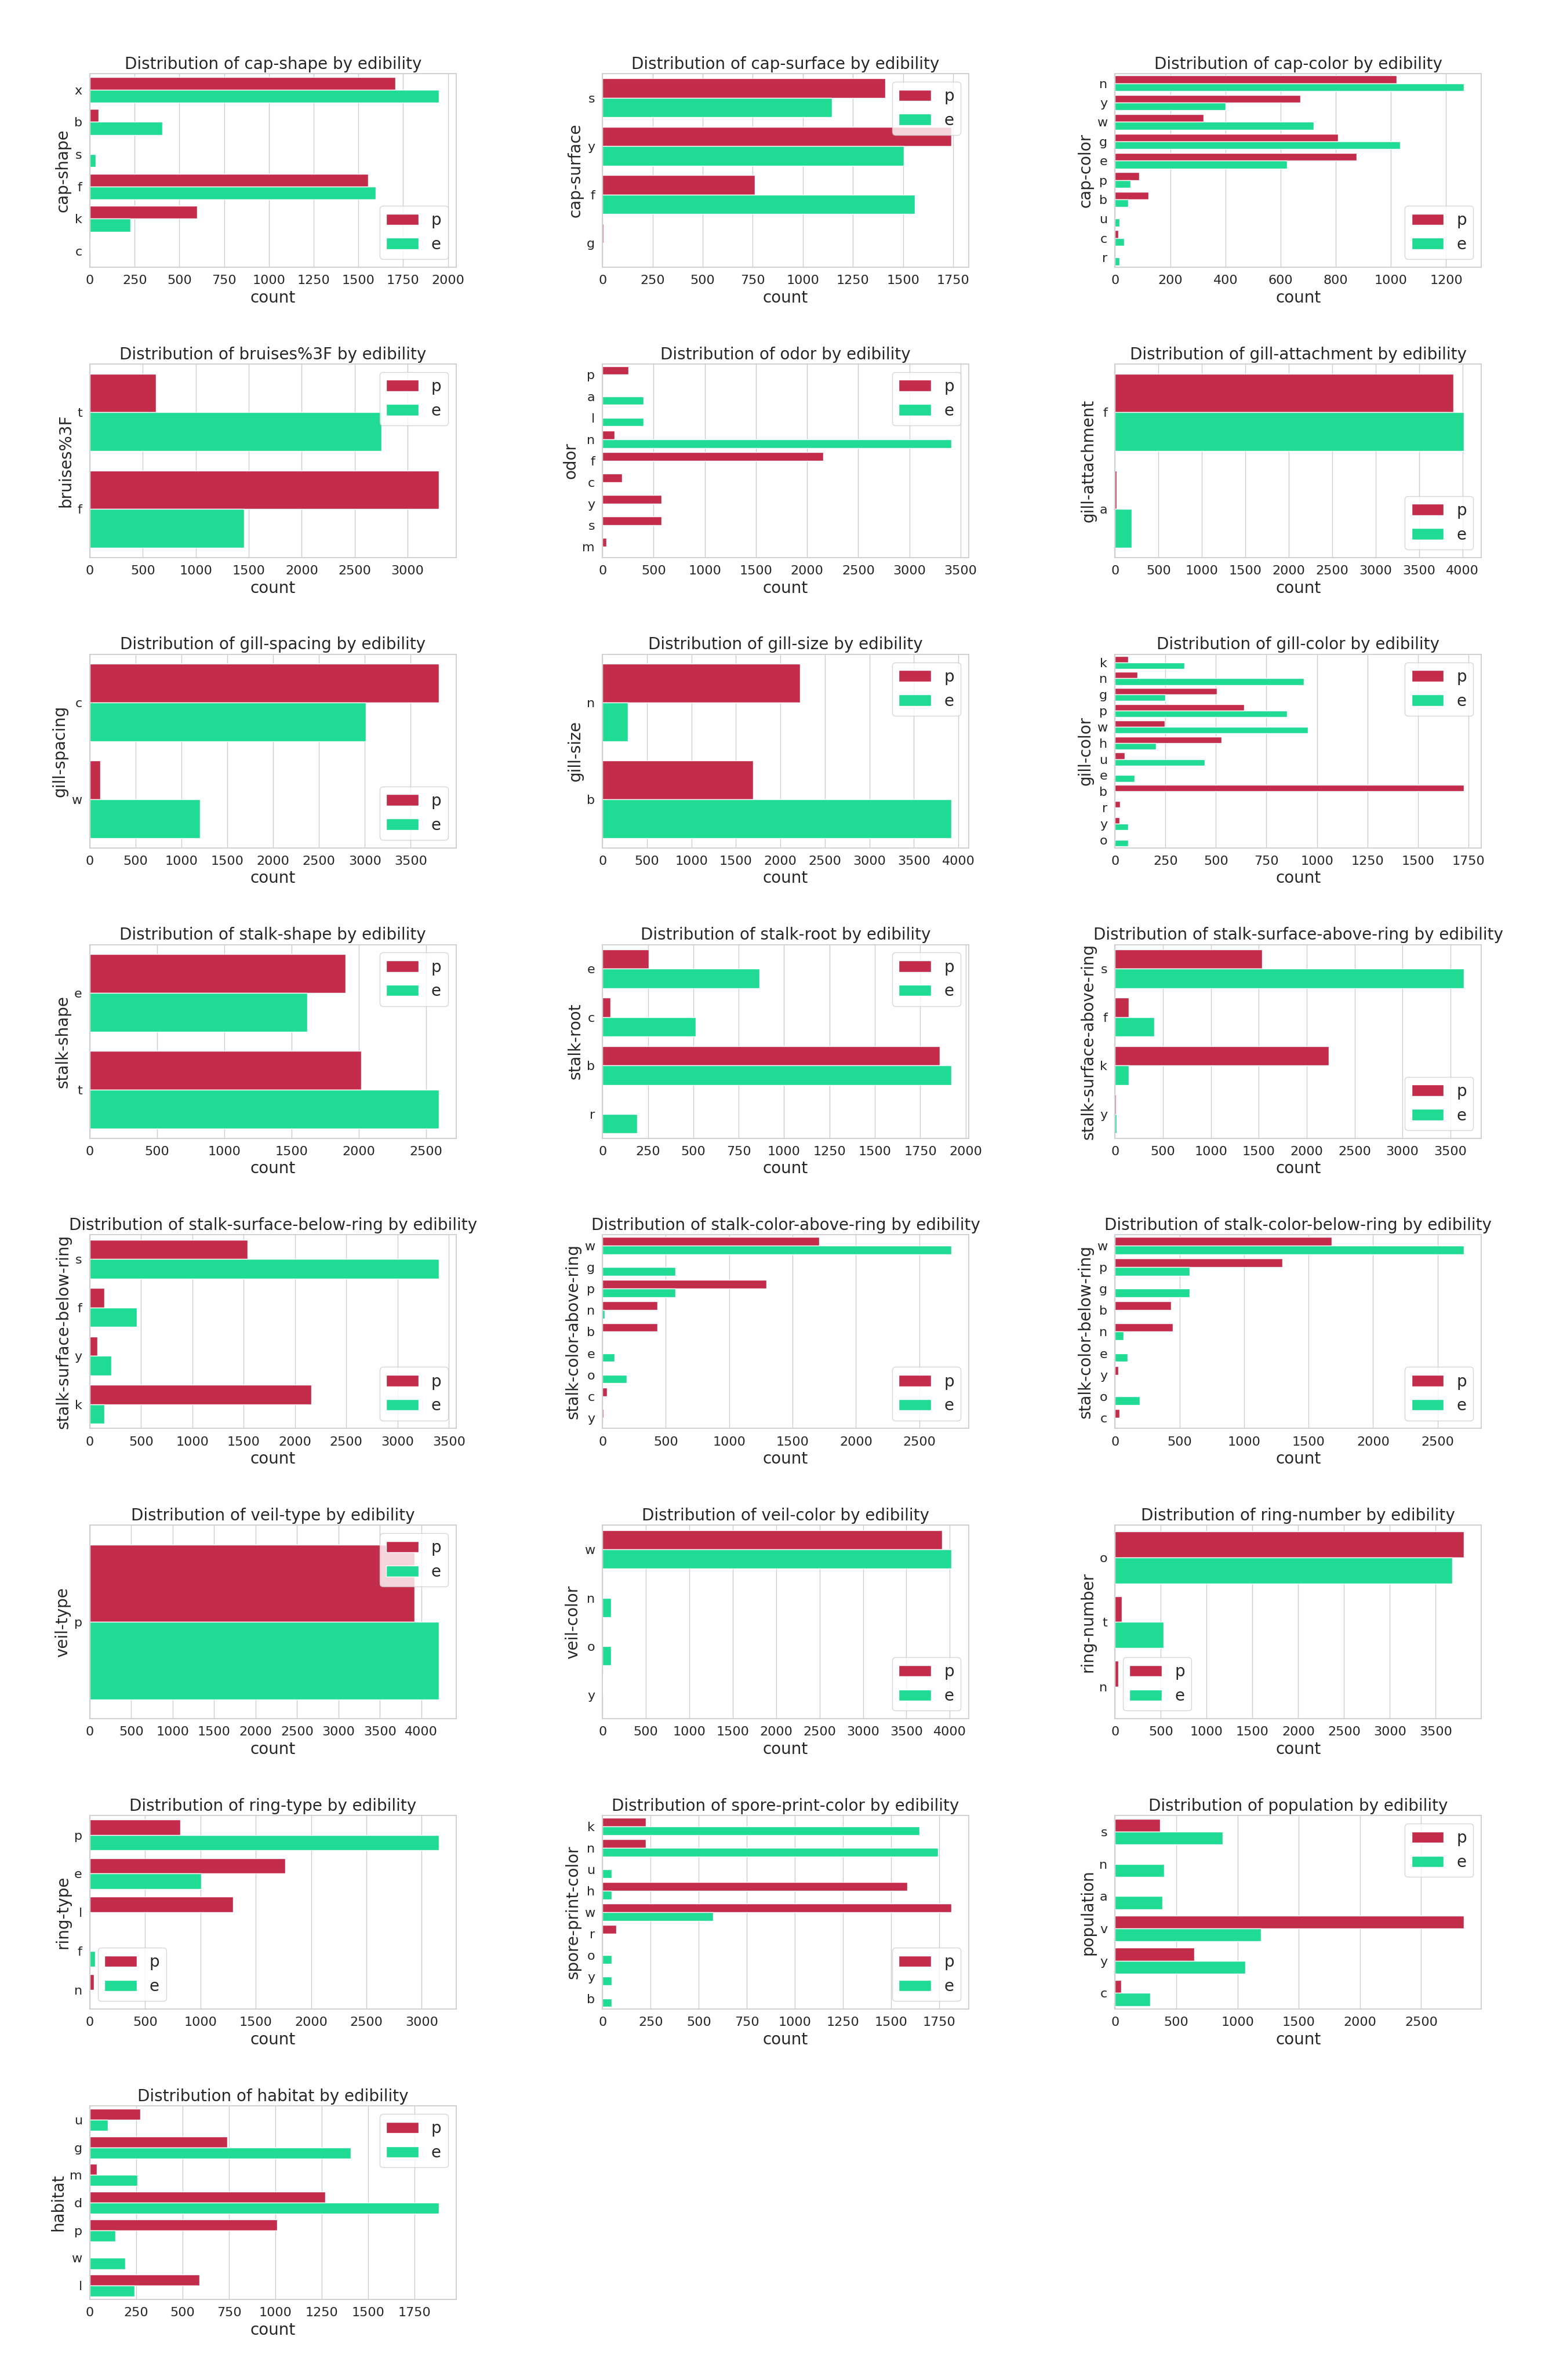
\includegraphics[scale=0.116]{visualize.jpeg}
	\caption{Visualization of data of all categories}
	\label{fig}
\end{figure}


\section{Training Model}
To train the model, the data set must first be divided into features and labels, denoted by variables X and y. The y variable is determined to be the "class" feature because it is the dependent variable in this case. X is the remaining features. Using the Sklearn library we were then able to split the data into training and test sets used to train and fit the model. For this we chose a 70/30 split where 70\% of the data goes into train sets and 30\% of the data goes into test sets. Next, a random forest classifier with 10 estimators was created. We trained the model on the training data set using the fit function and training sets found earlier as parameters. Then with the trained model we were finally able to make predictions using the predict function provided by the Sklearn library.
\\
\\
Additionally, we used k-fold cross validation with 10 folds to select hyperparameters and to improve the accuracy of our model. This was again done with Sklearn. In k-fold validation k-1 folds are used as training data, which is then validated on the remaining part of the data. The performance measure is the is the average of the values computed in the loop, which will be discussed in the next section.

\section{Accuracy of Model}
Below are the confusion matrices for the model based on the training data and on the test data. A test-train split of $0.3$ is used for a total of  Because the model correctly identifies all instances in the dataset, we acheive an Accuracy of $100\%$ .
Random forest achieves perfect accuracy on this data set because some of the features are very highly correlated with the target class (poisonous vs edible). Many of these features have exceptionally low p-values when compared to the target class. Additionally many features have a feature importance greater than $0.1$ (ring-type, odor, spore-print-color, gill-color, gill-size - see Table 3). The combination of these features creates enough separability between the two binary classes that the model is able to perfectly distinguish between them. 

\begin{table}[h]
    \centering
    \begin{tabular}{|c|c|c|} \hline 
         &  y=1& y=0\\ \hline 
          ŷ =1&  2935& 0\\ \hline 
           ŷ=0&  0& 2751\\ \hline
    \end{tabular}
    \caption{Confusion matrix for training set}
    \label{tab:my_label}
\end{table}
 
 \begin{table}[h]
     \centering
     \begin{tabular}{|c|c|c|} \hline 
          &  y=1& y=0\\ \hline 
          ŷ =1&  1273& 0\\ \hline 
          ŷ =0&  0& 1165\\ \hline
     \end{tabular}
     \caption{Confusion matrix for test set}
     \label{tab:my_label}
 \end{table}

\begin{table}[h]
    \centering
    \begin{tabular}{|c|c|} \hline 
    Feature                 &  Importance\\ \hline
    ring-type                 &  0.155227\\ \hline
    odor                      &  0.143699 \\ \hline 
    spore-print-color         &  0.127049 \\ \hline 
    gill-color                &  0.112346 \\ \hline 
    gill-size                 &  0.092441 \\ \hline 
    stalk-root                &  0.082176 \\ \hline 
    population                &  0.054051 \\ \hline 
    stalk-surface-below-ring  &  0.045363 \\ \hline 
    habitat                   &  0.038348 \\ \hline 
    stalk-shape               &  0.025254 \\ \hline 
    gill-spacing              &  0.023300 \\ \hline 
    ring-number               &  0.022665 \\ \hline 
    cap-color                 &  0.019705 \\ \hline 
    stalk-color-below-ring    &  0.012749 \\ \hline 
    cap-shape                 &  0.011328  \\ \hline 
    bruises\%3F               &   0.009085  \\ \hline 
    stalk-color-above-ring    &  0.007656 \\ \hline 
    cap-surface               &  0.006526 \\ \hline 
    stalk-surface-above-ring  &  0.005640 \\ \hline 
    veil-color                &  0.005394 \\ \hline 
    veil-type                 &  0.000000 \\ \hline 
    gill-attachment           &  0.000000   \\ \hline 

    \end{tabular}
    \caption{Feature importance for each of the 22 features}
    \label{tab:my_label}
\end{table}


\newpage
\section{Conclusion}
Random forests are a very powerful class of models that can be used to great effect in many classification tasks. As illustrated here, if the data set contains sufficient separation between classes, then the Random Forest algorithm can achieve very high accuracy with relatively low computational complexity (The model used here only uses 10 total estimators). The Audubon Society Field Guide to North American Mushrooms (the source from which this data was extracted) states that there are no simple rules for determining the edibility of a mushroom (\url{https://www.kaggle.com/datasets/joebeachcapital/mushrooms/data}{ }), however, machine learning models such as this one can easily extract 'rules' without over-fitting which always work (in this particular data set).


\medskip


\textbf{Link to GitHub:} \\
\url{https://github.com/bsweyand/COMP-562-Final-Project.git}
\end{document}
